\chapter{Background\label{cha:chapter3}}

\section{Neural Networks}
\begin{figure}[h]
\centering
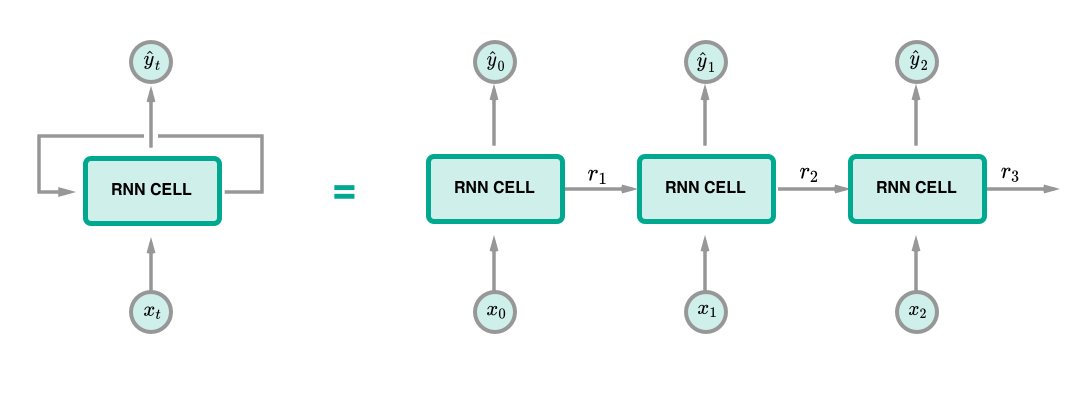
\includegraphics[width=0.8\textwidth]{sketch/rnn_unfold}
\caption{RNN Structure}
\label{fig:rnn_unfold}
\end{figure}

\subsection{Learning Algorithms}
\subsubsection{Loss functions}
\subsubsection{SGD}
\subsubsection{ADAM}
\subsubsection{Backpropagation Through Time}
\subsubsection{Vanishing and exploding gradient}

\subsection{CNNs}
\subsection{RNNs}

\section{Explainability of Neural Networks}
Neural networks have become one of major machine learning algorithms used in many applications, for example computer vision and medicine. Despite those achievements, they are still considered as a blackbox process that is  difficult to interpret its results or find evidences that the networks use to make such accurate decisions for further analysis.

Moreover, it is always important to verify whether the trained network properly utilize data or what information it uses to make decisions. Literatures usually call this process as ``Explainability''.  \cite{BachAnalyzingclassifiersFisher2016} show that there are situations that the networks exploit artifacts in the data to make decisions. This discovery emphasizes the importance of having explainable neural networks, not to mention the fact that we are applying more and more neural networks to domains that human's life involved, such as medicine or self-driving car.

There are 2 approaches towards explaining neural network, namely \textit{Global} and \textit{Local} analysis. Given a  classification problem of $\mathcal{C}$ classes classification problem and a trained network, global method aims to find an input $\patvector{x}^*$ that is the most representative to a class $c \in \mathcal{C}$. ``Activation Maximization\cite{ErhanUnderstandingRepresentationsLearned2010}'' is such method.
$$
\patvector{x}^*  = \patarg{max}{\patvector{x}}  \mathbb{P}( c |\patvector{x},\theta)
$$

On the other hand, local analysis focuses on finding relevant information in $\patvector{x}$ that causes the network predicting class $c_i$.  For example, consider an image classification problems, we can interpret a pixel $x_i \in \patvector{x}$ as a feature, this local analysis tries to find relevance score of each pixel in respect to the classification decision. This process usually results in heatmap intensity, often called relevance heatmap $R(\patvector{x})$.

The difference  between the 2 approaches can be analogously described by formulating questions as follows : Consider $\patvector{x}$ is an image in category ``car".
\begin{itemize}
	\item Global analysis : ``what does the usual car look like?"
    \item Local analysis : ``which area in the image make it look like car?" wheels, windows?
\end{itemize}

 \begin{figure}[!hbt]
\centering
\includegraphics[width=0.8\textwidth]{sketch/comparision_global_local}
\caption{Comparison between Global and Local Analysis}
\label{fig:comparision_between_global_and_local_analysis}
\end{figure}

In the following, I will leave content of global analysis aside and discuss  only approaches in local analysis further.  In particular, I will start with properties that literatures usually use to analysis goodness of a method. These properties can imply the quality of relevance heatmap. Then, I will discuss  3 methods, namely Sensitivity Analysis,  Simple Taylor Decomposition and Layer-wise Relevance Propagation.

Consider $f(\patvector{x})$ is an output from a neural network classifier that is corresponding to the class prediction, for example the value at the final layer before applying softmax function.
\begin{definition} Conservation Property
\begin{align*}
	\forall \patvector{x} : f(\patvector{x}) = \sum_i R_i
\end{align*}
Sum of relevance score of each pixel $x_i$ should equal to the total relevance that the network outputs.

\end{definition}
\begin{definition} Positivity Property
\end{definition}
\begin{definition} Consistency
\end{definition}

\subsection{Sensitivity Analysis}
Sensitivity analysis\cite{SimonyanDeepConvolutionalNetworks2013} is a local analysis that derives relevance $R_i$ of pixel $x_i$, from the partial derivative of $f(\patvector{x})$ respect to $x_i$. In particular, literature usually formulates the calculation as 

\begin{align*}
	R_i =
	 \bigg( \frac{\partial f(\patvector{x})}{ \partial x_i } \bigg)^2
\end{align*}

Hence, 
\begin{align*}
	\sum_i R_i = || \nabla f(\patvector{x}) ||^2
\end{align*}

Although this technique can be easily implemented via automatic differentiation provided in modern deep learning frameworks, such as TensorFlow\cite{AbadiTensorFlowLargeScaleMachine2016}, the derivation of $\sum_i R_i$ above implies that sensitivity analysis instead seeks to explain $R_i$ from the aspect of variation magnitudes, not the actual relevance quantity.

\subsection{Guided Backpropagation}
Guided backpropagation is a extended version of sensitivity analysis where gradients are propagated in a controlled manner. It is designed specifically for neural network using piecewise linear activations. In particular, Springenberg et al.\cite{SpringenbergStrivingSimplicityAll2014e} reformulate the definition  of ReLU function as:
\begin{align*}
	\sigma(x) = x \mathbbm{1}[ x > 0 ],
\end{align*}
where $\mathbbm{1}[ \cdot ]$  is an indicator function. With the new formulation, \cite{SpringenbergStrivingSimplicityAll2014e} proposes a new derivative of a ReLU neuron $j$ as:
\begin{align*}
	\frac{\partial_* f(\patvector{x}) }{ \partial a_j } = \mathbbm{1}\bigg[a_j > 0 \bigg] \mathbbm{1}\bigg[ \frac{ \partial f(\patvector{x}) }{ \partial a_j } > 0 \bigg] \frac{ \partial f(\patvector{x}) }{ \partial a_j } 
\end{align*}
The 2 indicator functions control whether original gradients are propagated back, hence the name ``Guided Backpropagation''. Hence, the relevance score for $x_i$ is:

\begin{align*}
	R_i = \bigg( \frac{ \partial_* f(\patvector{x}) }{ \partial x_i }  \bigg)^2
\end{align*}

With this result, one can see that $x_i$ is relevant to the problem if activations $a_j$ that it supplies are active and positively contribute to $f(\patvector{x})$.


\subsection{Simple Taylor Decomposition}
This method decomposes $f(\patvector{x})$ into terms of relevance scores $R_i$ via Taylor Decomposition. Formally, 

\begin{align*}
	f(\patvector{x}) 	&= f(\tilde{\patvector{x}}) + \sum_{i} \underbrace{\frac{\partial f }{ \partial x_i } \Bigg|_{x_i = \tilde{x}_i}  ( x_i - \tilde{x}_i ) }_{R_i} + \zeta, 
\end{align*}
where $\zeta$ is the second and higher order terms of Taylor series and $\tilde{\patvector{x}}$ is a root point where $f(\tilde{\patvector{x}}) = 0 $.  To find such  $\tilde{\patvector{x}}$, one need to optimize :
$$
\underset{\xi \in \mathcal{X} }{\text{min}}  || \xi - \patvector{x} ||^2 \hspace{2cm}  \text{such that}\  f(\xi) = 0,
$$
where $\mathcal{X}$ represents the input distribution. However, this optimization is time consuming  and $\xi$ might potentially be close to or diverge from $\patvector{x}$ leading to non informative $R_i$.
%, not to mention information leak to $ O(\patvector{x}^T\patvector{x})$.

Nonetheless, Montavon et al.\cite{MontavonMethodsInterpretingUnderstanding2017} demonstrate that  neural networks whose activations $\sigma(x)$ are piecewise linear functions  with $\sigma(tx) = t\sigma(x) ,\forall t \ge 0$ property, for example a deep Rectified Linear Unit (ReLU) network without biases, $\tilde{\patvector{x}}$ can be found in  approximately the same flat region as $\patvector{x}$, $\tilde{\patvector{x}} = \underset{\epsilon \rightarrow 0 }{\lim} \epsilon \patvector{x}$, yielding

 $$\frac{\partial f(\patvector{x})}{\partial x_i}\bigg|_{\patvector{x}={\tilde{\patvector{x}}}} = \frac{\partial f(\patvector{x})}{\partial x_i}\bigg|_{\patvector{x}={\patvector{x}}} $$

Hence, the decomposition can be simplified to :
\begin{align*}
	f(\patvector{x}) &= \sum_{i} \underbrace{\frac{\partial f(\patvector{x})}{\partial x_i}\bigg|_{\patvector{x}={\patvector{x}}}  x_i}_{ R_i } 
\end{align*} 

Moreover, the result suggests the relationship between sensitivity analysis and Taylor decomposition. Specifically, $x_i$ has high relevance score if $x_i$ activates and its variation positively affects $f(x)$ and vice versa.


%it is ensured that $$. Hence,  this decomposition can be simplified to :
%\begin{align*}
%	f(\patvector{x}) = 
%\end{align*}
%%


\subsection{Layer-wise Relevance Propagation}
The methods mentioned so far derive $R_i$ directly from $f(\patvector{x})$ and do not  use important knowledge about the network itself, such as architecture or activation values. Alternatively, Bach et	 al.\citep{BinderLayerwiseRelevancePropagation2016} propose Layer-wise Relevance Propagation(LRP) framework that leverages this known information to distribute relevance scores to $x_i$. In particular, LRP propagates relevance scores backward from layer to layer, similar to the back-propagation algorithm of gradient descent.

\afterpage{

 \begin{figure}[!hbt]

\begin{center}
	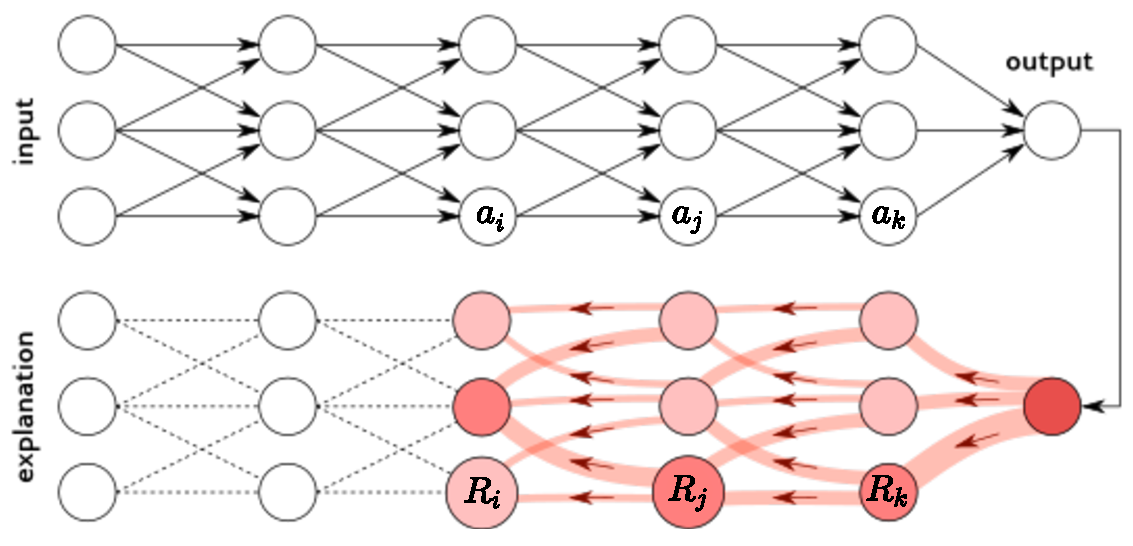
\includegraphics[width=0.8\textwidth]{sketch/lrp_graph}
	\caption[The LOF caption]{LRP Framework\footnotemark}
	\label{fig:lrp_graph}
\end{center}

\end{figure}
\footnotetext{Source: \url{http://heatmapping.org}}
}

Consider the neural network illustrated in \addfigure{\ref{fig:lrp_graph}}. $R_j$ and $R_k$ are relevance score of  neurons $j,k$ in successive layers.  \cite{BinderLayerwiseRelevancePropagation2016} formulates the general form of relevance propagation as :

\begin{align} \label{eq:general_lrp_rj}
	R_j = \sum_{k} 	\delta_{j\leftarrow k} R_{k} ,
\end{align}

where $\delta_{j\leftarrow k}$ defines a proportion that  $R_{k}$ contributes to $R_j$. Consider further that activity $a_k$ of neuron $k$ is computed by 
\begin{align*}
	a_k = \sigma \bigg( \sum_{j} w_{jk} a_j + b_k \bigg),
\end{align*} 
where $w_{jk}, b_k$ are the corresponding weight and bias between neuron $j$ and $k$, and $\sigma$ is a monotonic increasing activation function. \cite{BinderLayerwiseRelevancePropagation2016} suggests 
\begin{align}
	\delta_{j\leftarrow k} = \alpha\frac{a_j w_{jk}^+}{\sum_{j} a_jw_{jk}^+} - \beta\frac{a_j w_{jk}^-}{\sum_{j} a_jw_{jk}^-},
\end{align}
where $w_{jk}^+$, $w_{jk}^-$ are $\max(0, w_{jk})$, $\min(0, w_{jk})$, and $\alpha$,  $\beta$ are parameters with $\alpha-\beta = 1$ condition. Together with Equation \ref{eq:general_lrp_rj}, \cite{BinderLayerwiseRelevancePropagation2016} calls $\alpha\beta$-rule.

\begin{align}
	R_j = \sum_{k} 	\bigg( \alpha\frac{a_j w_{jk}^+}{\sum_{j} a_jw_{jk}^+} - \beta\frac{a_j w_{jk}^-}{\sum_{j} a_jw_{jk}^-} \bigg )  R_{k}
\end{align}


%TODO : how LRP ensure conservation property?
This $\alpha\beta$-rule ensures that conservation property is satisfied as $f(\patvector{x})$ is distributed through the network. 
\begin{align*}
	\sum_{i} R_i = 	\sum_{j} R_j = 	\sum_{k} R_k = f(\patvector{x})
\end{align*}

Moreover, if we rewrites  $\alpha\beta$-rule as 
$$
	R_j = \sum_{k}  \frac{a_j w_{jk}^+}{\sum_{j} a_jw_{jk}^+} \hat{R}_{k} + \frac{a_j w_{jk}^-}{\sum_{j} a_jw_{jk}^-} \check{R}_{k},
$$ 
where $\hat{R}_{k}  = \alpha R_{k}$ and  $\check{R}_{k} = -\beta R_{k} $. Then, we can intuitively interpret this propagation as 

\begin{quote}
``Relevance $\hat{R}_k$'' should be redistributed to the lower-
layer neurons $\{a_j\}_j$ in proportion to their excitatory effect on $a_k$. ``Counter-relevance'' $\check{R}_k $ should be redistributed to the lower-layer neurons $\{a_j\}_j$ in proportion to their inhibitory effect on $a_j$
	- Section 5.1 \cite{MontavonMethodsInterpretingUnderstanding2017}
\end{quote} 

However, it seems that there is no clear relationship between values of $\alpha,\beta$ and the structure of the heatmap. \cite{MontavonMethodsInterpretingUnderstanding2017, BinderLayerwiseRelevancePropagation2016} demonstrate that the values are depend on the architecture of the network. In particular, \cite{MontavonMethodsInterpretingUnderstanding2017} observes that $\alpha=1, \beta=0$ works well for deep architectures, such as GoogleNet\cite{SzegedyGoingDeeperConvolutions2014}, while  $\alpha=2, \beta=1$ for shallower architectures, such as BVLC CaffeNet\cite{JiaCaffeConvolutionalArchitecture2014}.



\begin{algorithm}[H]
$f(\patvector{x}), \{ \{a\}_{l_1}, \{a\}_{l_2}, \dots, \{a\}_{l_n}\}$ = \text{forward\_pass}($\patvector{x}, \patvector{\theta}$)\;
$R_k = f(\patvector{x})$\;
 \For{ $\text{layer} \in \text{reverse}(\{l_1, l_2, \dots, l_n\})$}{
$ \text{prev\_layer} \leftarrow \text{layer}  - 1$ \;
	\For{ $j \in $ neurons(prev\_layer), $k \in$ neurons(layer)}{
		$R_j \leftarrow \alpha\beta$-rule$(R_k, \{a\}_j, \{ w \}_{j,k} )$\;
	}
 }
 \caption{LRP Algorithm}
 \label{algo:lrp}
\end{algorithm}

%TODO: Heatmap comparision Figure sensitivity, simple taylor, lrp


\section{Deep Taylor Decomposition}
Deep Taylor Decomposition(DTD) is a explanation technique that decomposes $R_k$ as a sum of $R_j$ from previous layer using Simple Taylor Decomposition. Montavon et al.\cite{MontavonExplainingnonlinearclassification2017} proposes the method to explain decisions of neural networks with piece-wise linear activations. Similar to LRP, DTD decomposes $R_k$ and propagates the quantity backward to $R_J$. In particular, $R_k$ is decomposed as follows :


% In fact, it can be shown that LRP's propagation rule is equivalent to one of DT's rules.


 \begin{align} \label{eq:tl_rj}
 R_k = R_k \bigg|_{ \tilde{\patvector{a}}_j } + \sum_{ j } 	\frac{\partial  R_k }{ \partial a_j } \bigg|_{ a_j = \tilde{a}_j } ( a_j - \tilde{a}_j ) + \zeta_k
 \end{align}

Assume further that there exists a root point $\tilde{\patvector{a}}_j$ such that $R_k = 0$, and the second and higher terms $\zeta_k = 0 $. Then, Equation \ref{eq:tl_rj} is simplified to
\begin{align} \label{eq:R_k_sum}
 R_k = \sum_{ j } \underbrace{	\frac{\partial  R_k }{ \partial a_j } \bigg|_{ a_j = \tilde{a}_j }  ( a_j - \tilde{a}_j ) }_{ R_{j \leftarrow k } }
\end{align}

Moreover, as the relevance propagated back, \cite{MontavonExplainingnonlinearclassification2017} shows that $R_j$ is an aggregation of $R_{j\leftarrow k}$ from neuron $k$ in the next layer that neuron $j$ contributes to. Formally, this is
\begin{align} \label{eq:R_j_sum}
	R_j = \sum_{k} R_{j\leftarrow k}
\end{align}

Combining Equation \ref{eq:R_k_sum} and \ref{eq:R_j_sum} yields :
\begin{align} \label{eq:rj_equal_rk}
	R_j &= \sum_{k} R_{j\leftarrow k} \nonumber \\
\sum_{j}	R_j &= \sum_{j} \sum_{k} R_{j\leftarrow k}\nonumber\\
\sum_{j}	R_j &= \sum_{k} \sum_{j} R_{j\leftarrow k} \nonumber\\
\sum_{j}	R_j &= \sum_{k}  R_{k}
\end{align}

Demonstrated by \cite{MontavonExplainingnonlinearclassification2017}, Equation \ref{eq:rj_equal_rk} holds for all $j, k$ and all subsequent layers. Hence, this results in  conservation property which guarantee that no relevance loss during the propagations.
\begin{align}
\sum_i 	R_{i} = 	\dots = \sum_j R_{j} = \sum_k R_{k} = \dots =  f(\patvector{x})
\end{align}
 
 
%\begin{figure}[h]
%\centering
%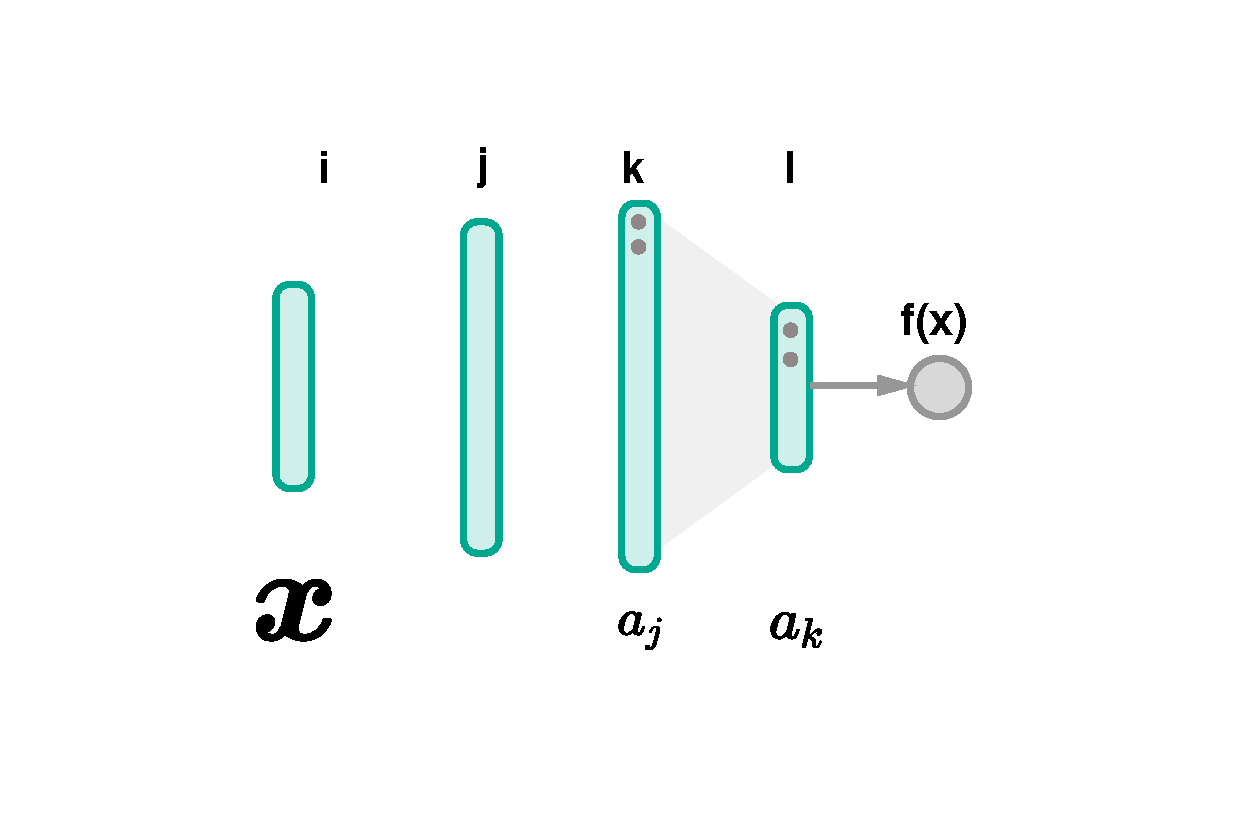
\includegraphics[width=0.8\textwidth]{sketch/deep_tayloy_decomposition_toy}
%\caption{A Simple network}
%\label{fig:deep_tayloy_decomposition_toy}
%\end{figure}

To find a root point $\tilde{\patvector{a}}_j$, consider a neural network whose $R_k$ is computed by :
\begin{align}\label{eq:r_k_deep_taylor}
R_k = \text{max}\ \bigg(0, \sum_{j} a_j w_{jk}  + b_k \bigg),
\end{align}
where $b_k \le 0 $.

One can see that  there are  2 cases to be analyzed, namely $R_k = 0$ and $R_k \ge 0$. For $R_k=0$,  $\patvector{a}_j$ is already the root point. For the latter, one can find such point by performing  line search in  a direction $\patvector{v}_j$ and magnitude $t$.
\begin{align}\label{eq:root_aj_aj}
\tilde{a}_j = a_j - t v_j,
\end{align}
The root point is then the intersection point between Equation \ref{eq:root_aj_aj} and \ref{eq:r_k_deep_taylor}. Hence,
\begin{align}
  0 &= 	\sum_{j} (a_j - t v_j) w_{jk}  + b_k\\
%  0 &= \sum_{j} a_j w_{jk} - t v_j w_{jk}  + b_k\\
  t \sum_{j} v_j w_{jk} &= R_k \\
  t &= \frac{R_k}{\sum_{j} v_j w_{jk}} \\
\end{align}

Therefore, $R_j$ can be computed by :
\begin{align}
R_j &= \sum_k	\frac{\partial  R_k }{ \partial a_j } \bigg|_{ a_j - \tilde{a}_j }  ( a_j - \tilde{a}_j ) \\
&=	\sum_k w_{jk} tv_j \\
&=	\sum_k \frac{ v_j w_{jk}   }{\sum_{j} v_j w_{jk}}  R_k
\end{align}

Noticing here is that $\tilde{\patvector{a}}_j$ is not necessary the closest point to the line $R_k=0$ in Euclidean distance, because  $\tilde{\patvector{a}}_j$  might not be in the same domain as $\patvector{a}_j$, hence $v_j$ needs to be chosen according to the domain of $\patvector{a}_j$. Consider an example on \addfigure{\ref{fig:root_point_illus}}, if $a_j \in \mathbb{R}^+$, then $\widetilde{a_j}$ must be also in $\mathbb{R}^+$.   In the following, I will summarize how $\patvector{a}_j$ can be computed for each domain of $\patvector{a}_j$.

\begin{figure}[h]
\centering
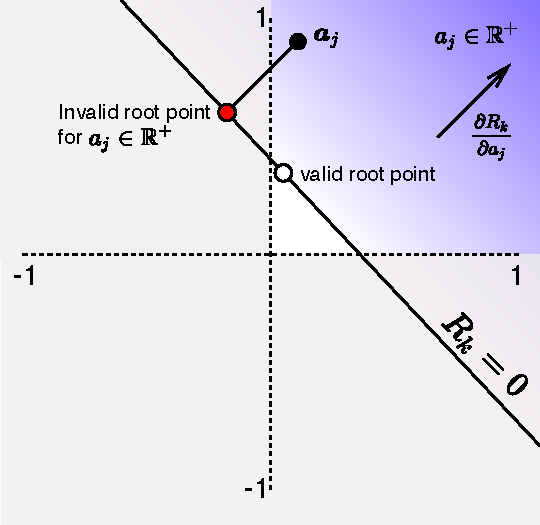
\includegraphics[width=0.4\textwidth]{sketch/invalid_root_point_example}
\caption{An illustration of $R_k$ functional view and root point candidates}
\label{fig:root_point_illus}
\end{figure}

\subsubsection{Case $a_j \in \mathbb{R}$ : $w^2$-rule}

Trivially, the search direction $v_j$ is just the direction of gradient $\frac{\partial  R_k^{(l+1)} }{ \partial a_j^{(l)} }$:
\begin{align*}
	v_j = w_{jk}
\end{align*}

Hence, 
\begin{align*}
	R_j &=	\sum_k \frac{ w_{jk}^2  }{\sum_{j} w_{jk}^2}  R_k
\end{align*}

\subsubsection{Case $a_j \ge 0$ : $z^+$-rule}
The root point is on the line segment $( \patvector{a_j} \mathbbm{1}\{ w_{jk}  < 0 \}, \patvector{a_j} )$. In particular, as shown on \addfigure{\ref{fig:zplus_rule_cases}}, $R_k$ has a root at $\patvector{a_j} \mathbbm{1}\{ w_{jk}  < 0 \}$, because of:
\begin{align}	
R_k &= \max \bigg( \sum_j a_j w_{jk } + b_k, 0 \bigg) \\
&=  \max \bigg( \sum_j a_j \mathbbm{1}\{ w_{jk}  < 0 \} w_{jk} + b_k, 0 \bigg) \\
&=  \max \bigg(\sum_j a_j  w_{jk}^- + b_k , 0\bigg) \\
&= 0 \label{eq:zplus_rk_zero}
\end{align}
The last step uses the fact that $a_j \in R^+$ and $b_k \le 0$ from the assumption. Hence, the search direction is:
\begin{align*}
	v_j &= a_j - a_j \mathbbm{1}\{ w_{jk}  < 0 \} \\
	&= a_j \mathbbm{1}\{ w_{jk}  \ge 0 \}
\end{align*}

\begin{figure}[!htb]
\centering
\subfloat[]{%
       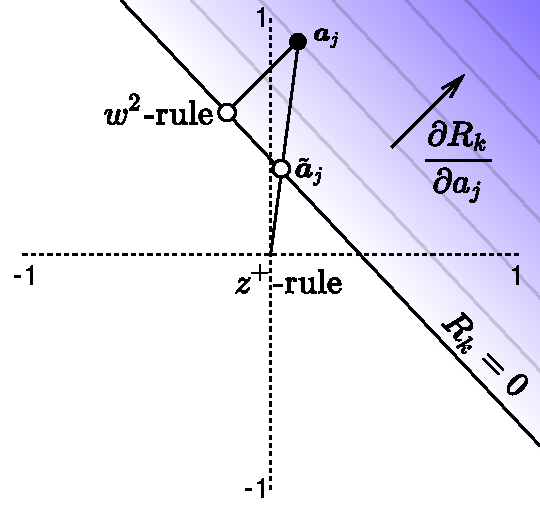
\includegraphics[width=0.4\textwidth]{sketch/zplus_rule_case_1}
     }
%     \hfill
     \subfloat[]{%
       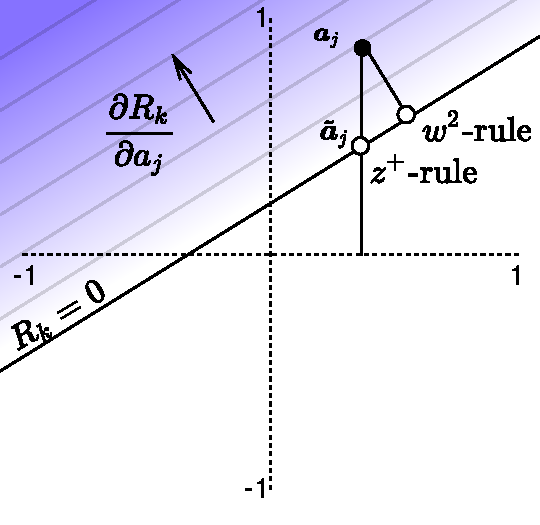
\includegraphics[width=0.4\textwidth]{sketch/zplus_rule_case_2}
     }
\caption{$R_k$ functional view and root points from $z^+$-rule}
\label{fig:zplus_rule_cases}
\end{figure}



Therefore, 
\begin{align*}
		R_j &=	\sum_k \frac{ w_{jk} a_j \mathbbm{1}\{ w_{jk}  \ge 0 \}  }{\sum_{j} w_{jk} a_j \mathbbm{1}\{ w_{jk}  \ge 0 \} }  R_k\\
		&=	\sum_k  \frac{ a_j  w_{jk}^+   }{\sum_{j}  a_j w_{jk}^+  }  R_k
\end{align*}

Moreover, one can also see that $z^+$-rule is equivalent to LRP's $\alpha\beta$-rule when $\alpha=1, \beta=0$. 


\subsubsection{Case $l_j \le a_j \le h_j$ where $l_j \le 0 < h_j $ : $z^\beta$-rule}
In this case, the root point is on the line segment $( l_j \mathbbm{1}\{ w_{jk}  \ge 0 \}  + h_j \mathbbm{1}\{ w_{jk}  \le 0 \}  , a_j ) $. One can show that 
\begin{align}
R_k &= \max \bigg( \sum_j a_j w_{jk } + b_k, 0 \bigg) \\
&=\max \bigg( \sum_j (l_j \mathbbm{1}\{ w_{jk}  \ge 0 \}  + h_j \mathbbm{1}\{ w_{jk}  \le 0 \} ) w_{jk } + b_k, 0 \bigg) \\
&= \max \bigg( \sum_j l_j w_{jk }^+   + h_j w_{jk }^-  + b_k, 0 \bigg) \\
&= 0
\end{align}

Hence,  the search direction is 
\begin{align*}
	v_j &= a_j - \tilde{a}_j \\
	&=a_j  - l_j \mathbbm{1}\{ w_{jk}  \ge 0 \}  - h_j \mathbbm{1}\{ w_{jk}  \le 0 \}
\end{align*}

\addfigure{\ref{fig:zbeta_rule_cases}} illustrates details of the search direction. Therefore, 
\begin{align*}
		R_j &=	\sum_k \frac{ w_{jk}  (a_j  - l_j \mathbbm{1}\{ w_{jk}  \ge 0 \}  - h_j \mathbbm{1}\{ w_{jk}  \le 0 \}) }{\sum_{j} w_{jk}  (a_j  - l_j \mathbbm{1}\{ w_{jk}  \ge 0 \}  - h_j \mathbbm{1}\{ w_{jk}  \le 0 \}) }  R_k\\
		&=	\sum_k  \frac{ a_j  w_{jk} - l_j w_{jk}^- - h_j w_{jk}^+  }{\sum_{j}   a_j  w_{jk} - l_j w_{jk}^- - h_j w_{jk}^+  -}  R_k
\end{align*}

\begin{figure}[!htb]
\centering
\subfloat[]{%
       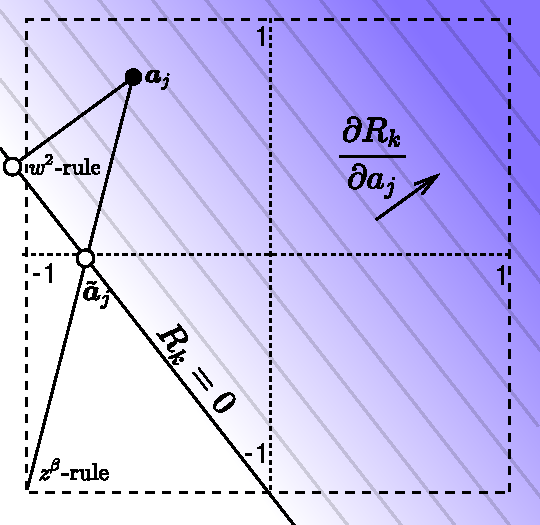
\includegraphics[width=0.4\textwidth]{sketch/zbeta_rule_case_1}
     }
%     \hfill
     \subfloat[]{%
       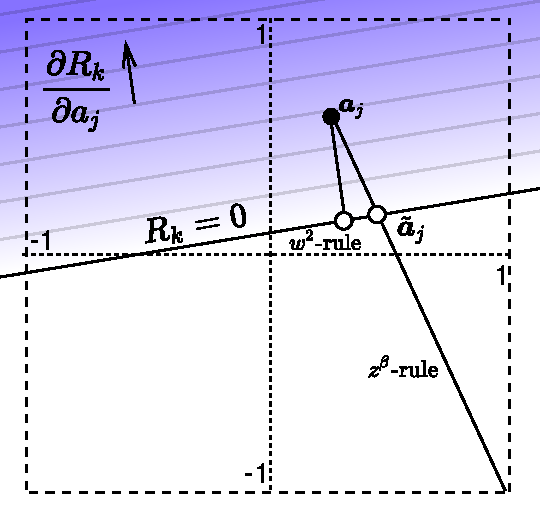
\includegraphics[width=0.4\textwidth]{sketch/zbeta_rule_case_2}
     }
\caption{$R_k$ functional view and root points from $z^\beta$-rule with $-1 < a_j < 1$ }
\label{fig:zbeta_rule_cases}
\end{figure}


In summary, DTD is a theory for explaining nonlinear compuations of neural network through decomposing relevance score between successive layers. Its propagation rules ensures conservation property. Given the rules above, the relevance scores can be propagated using LRP Algorithm \ref{algo:lrp}.

Lastly, as DTD provides more general propagation rules than the $\alpha\beta$-rule from LRP, I will use DTD and LRP interchangeably throughout the thesis. In particular, it will be mentioned explicitly if $\alpha\beta$ is being used, otherwise the rule is a DTD's rule.  Table \ref{tab:lrp_deep_taylor_rules} concludes the details  when such DTD rules should be used.


\renewcommand{\arraystretch}{1}
\begin{table}[h]
\centering
\begin{tabular}{|l|l|}
\hline
\multicolumn{1}{|c|}{Input Domain} & \multicolumn{1}{c|}{LRP Propagation Rule} \\ \hline
$w^2$-rule : Real values,  $a_j \in R$ & \parbox{1cm}{
	\begin{align*}
		R_j =	\sum_k \frac{ w_{jk}^2  }{\sum_{j} w_{jk}^2}  R_k  	
    \end{align*}}
 \\ \hline
% &                                \\ \hline
$z^+$-rule : ReLU activations, $a_j \ge 0$    & \parbox{1cm}{\begin{align*}
R_j = \sum_k  \frac{ a_j  w_{jk}^+   }{\sum_{j}  a_j w_{jk}^+  }  R_k	
\end{align*}} \\ \hline
$z^\beta$-rule : Pixel Intensities, $ l_j \le a_j \le h_j$, $l_j \le 0 \le h_j$  & \parbox{1cm}{\begin{align*}
R_j = \sum_k  \frac{ a_j  w_{jk} - l_j w_{jk}^- - h_j w_{jk}^+  }{\sum_{j}   a_j  w_{jk} - l_j w_{jk}^- - h_j w_{jk}^+  -}  R_k	
\end{align*}}
               \\ \hline
\end{tabular}
\caption{LRP rules from Deep Taylor Decomposition} %TODO : ca
\label{tab:lrp_deep_taylor_rules}
\end{table}
\renewcommand{\arraystretch}{1}


%
%As a result,  
%
%To find $\tilde{\patvector{a}}_j$ that is in the same region as $\patvector{a_j}$, $v_j$ need to be derived  
%Noticing that $v_j$ is depend on domain of $a_j$
%
%%\begin{align*}
%%R_k = \sum_{	
%%\end{align*}
%





%For the latter, we need 


%
%To find a $\tilde{\patvector{a}}^{(l)}$, consider a neural network on  \addfigure{\ref{fig:deep_tayloy_decomposition_toy}}. The forward pass computations are defined as follows: 
%
%\begin{align*}
%a_j &= \text{max}( \sum_{ i } x_i w_{ij} + b_j, 0 )\\
%a_k &=\text{max}( \sum_{ j } a_j w_{jk} + b_k, 0 ) \\
%a_l &= \sum_{ k } a_k w_{kl} + b_l, 0 \\\\
%f(x)  &= \text{softmax}( \{  a_l \} )
%\end{align*}
%
%Here, the relevance score is the corresponding $a_k$ of the softmax output. 
%
%
%To find such a root 
%One remaining component is $\tilde{\patvector{a}}^{(l)}$. To derive such a root point $\tilde{\patvector{a}}^{(l)}$, we first assume that
%\begin{align}
%a_k^{(l+1)} = \max \bigg(0, \sum_j a^{(l)}_j w_{jk}^{(l+1)} + b_k \bigg),
%\end{align}
%with constraint $b_k \le 0$.



%It might seem challenging to find 
%
% leverages the 
%  into several functions. It uses Simple Taylor Decomposition to decompose $R_j^{(l+1)}$ into a sum 
% 
%  sdf propagation method that is developed for a specific type of neural networks. That is the networks using ReLU activations. As the name suggested, the method is built upon Simple Taylor Decomposition of relevance score between 2 connecting layers.
% 
% l